According to the WLCG IPv6 plan, Tier-2 sites shall have
their storage systems and perfSONAR installation
working in dual stack by the end of 2018. To this purpose, a ticketing
campaign via GGUS was launched in November 2017, targeting all WLCG Tier-2
sites managed by EGI, while for OSG sites the coordination for the
IPv6 deployment was delegated to OSG operations.

The text of the tickets explained the goals and the motivation for the
IPv6 deployment, and asked the sites to provide an estimated time
scale for the deployment and some details about the required
steps. The last step would be a check by perfSONAR and experiment
experts that the services are working as expected via IPv6.

The status of the tickets was periodically reviewed and questions from
the sites addressed by the experts in the HEPiX IPv6 working
group. The tickets are classified as {\it no reply} 
%(no reaction from the site)
, {\it on hold} 
%(the site has to wait for something outside of its control)
, {\it in progress} 
%(the deployment is ongoing) 
and {\it done}.
%(the deployment is completed and successfully tested). 
Following the decommissioning of the OSG operations team, the
information about OSG sites is now sourced from the LHC experiments
themselves. The status of the deployment at the start of October 2018, both globally and by
region, is depicted in figure~\ref{fig:t2depl}.
\begin{figure}[t]
\centering
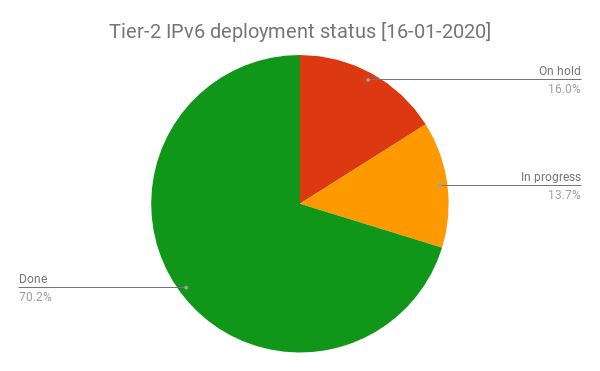
\includegraphics[width=6cm]{chart2}
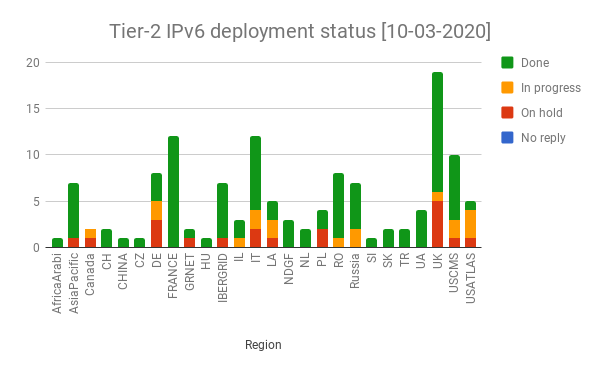
\includegraphics[width=6cm]{chart}
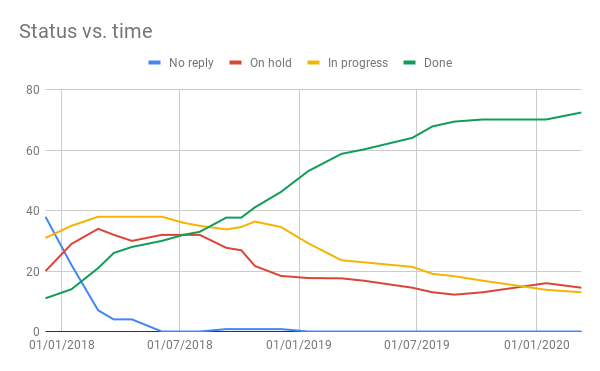
\includegraphics[width=6cm]{chart3}
\caption{(left) Tier-2 deployment status by site globally, (right) by region, and (centre) time evolution}
\label{fig:t2depl}
\end{figure}

The time evolution of the site status shows a steady increase of the
number of sites that have deployed IPv6. A detailed analysis of the
tickets shows that, in many cases, sites need to wait for the IPv6
deployment on site, which often depends on people different from the
WLCG site staff, while typically the deployment on the services
happens quickly and painlessly. It is interesting also to see the
fraction of the Tier-2 storage that is accessible via IPv6, which can
be simply calculated from the amount of storage space available to
each of the supported experiments (table~\ref{tab:t2stor}).
\begin{table}[h]
\centering
\caption{Fraction of Tier-2 storage available over IPv6}
\label{tab:t2stor}
\begin{tabular}{ccccc}
\hline
ALICE & ATLAS & CMS & LHCb & Global \\\hline
41\% & 33\% & 55\% & 33\% & 42\% \\\hline
\end{tabular}
\end{table}
Given that only very few sites declared that they will not be able to
meet the deadline, and that it is natural to expect more activity closer to
the deadline, it is expected that the Tier-2 deployment
goals will be successfully met.
